\documentclass[]{article}

% math packages
\usepackage{amsmath}
\usepackage{amsthm}
\usepackage{bm}

% for coloring in a table
%\usepackage[table,xcdraw]{xcolor}

% including graphics
\usepackage{graphicx}
\graphicspath{ {./images/} }

% drawing graphs
\usepackage{tikz-cd}
\usepackage{tikz}
\usetikzlibrary{shapes.geometric, arrows}
\tikzstyle{startstop} = [rectangle, rounded corners, minimum width=3cm, minimum height=1cm,text centered, draw=black, fill=red!10]
\tikzstyle{arrow} = [thick,->,>=stealth]

% hyperlinks
\usepackage{hyperref}

% some useful shortcuts
\DeclareMathOperator*{\argmax}{argmax}
\newcommand{\indep}{\perp\!\!\!\!\perp}
\newcommand{\blambda}{{\bm{\lambda}}}
\newcommand{\btheta}{{\bm{\theta}}}
\newcommand{\bpsi}{{\bm{\psi}}}

\newcommand{\by}{\mathbf{y}}

\usepackage{setspace}
\doublespacing

\usepackage{natbib}
\bibliographystyle{rusnat}

% Editing macros
\usepackage{color}
\newcommand\cmnt[2]{\qquad{{\color{red} \em #1---#2} \qquad}}
\newcommand\cmntM[1]{\cmnt{#1}{Miratrix}}
\newcommand\cmntC[1]{\cmnt{#1}{Che}}
\newcommand\awk{{{\color{red} {$\leftarrow$ Awkward phrasing}}\qquad}}
\newcommand\cmntMp[1]{{\color{red} $\leftarrow$ {\em #1 -Miratrix} \qquad}}



%opening
\title{On power analyses for individual site impacts in multisite trials}
\author{Jonathan Che \& Luke Miratrix}

\begin{document}

\maketitle


\section{Background}

Typically, researchers will power a multisite trial to ensure that a given design will achieve desired levels of power for the overall average treatment effect $\tau$ across all sites. 
In many applications, however, site stakeholders may be interested in estimating treatment effects $\tau_j$, $j = 1, \ldots, J$, at the individual sites as well.
To estimate site-level impacts, analysts typically use multilevel models (MLMs) to produce partially pooled estimates of the $\tau_j$.
For each site, these models ``borrow strength'' from the other sites, resulting in estimates $\hat{\tau}_j$ that are shrunken toward the estimated overall average treatment effect $\hat{\tau}$.
Standard Bayesian procedures may be used to construct credible intervals to conduct inference on these individual site-level effects.

The interpretation of these credible intervals requires some nuance, however.
There is an extensive literature concerning the construction of such intervals for individual site effects under shrinkage \citep{casella2012shrinkage}.
These intervals typically possess a so-called Empirical Bayes coverage property \citep{morris1983parametric}, i.e., they guarantee coverage for the collection of $\tau_j$ values \textit{on average} across all $J$ sites, not coverage for each individual $\tau_j$.
These guarantees may not be sufficient for stakeholders in multisite trials who would like to understand the effect of an experimental treatment at their particular site.
Overall, the question of inference for individual $\tau_j$ values in multilevel models remains fairly open \citep{armstrong2020robust}, with limited guidance about best practices.

\section{Objective}

In this paper, we provide guidance for analysts designing multisite trials with the knowledge that site stakeholders may be interested in individual site impact estimates.
We first demonstrate how naively applying standard power analysis methods to the multisite trial setting leads to unsatisfactory results, due to conflicts between Bayesian and Frequentist interpretations of coverage and power.
We then suggest a potential path forward.

% Similar power analyses have previously been conducted for the overall average treatment effect and cross-site variation in multisite trials \citep{raudenbush2000statistical}, but not for individual site-effect estimates, to the best of our knowledge.

% Two ideas to add:
% Idea 1: we're assuming exchangeability, so before the trial is run, everyone is the same to some extent?
% Idea 2: post-hoc power analyses are bad \href{https://statmodeling.stat.columbia.edu/2018/09/24/dont-calculate-post-hoc-power-using-observed-estimate-effect-size/}{says Gelman}

% We're doing a weird mix of pre- and post-trial stuff.
% In terms of coverage, things make sense.
% One idea: before we've run the analysis, what's the coverage of my intervals for sites with a true effect size of $\tau_j = 0.3$?
% Another idea: before we've run the analysis, what's the coverage of my intervals for sites with estimated $\hat{\tau}_j = 0.3$?

% In terms of power, things get weird.
% One idea: before we've run the analysis, what's the power of my procedure to detect effects at sites with $\tau_j = 0.3$?
% Another idea: before we've run the analysis, what's the power of my procedure to detect effects at sites with $\hat{\tau}_j = 0.3$?

% Is this second idea useful?
% Say I've run the trial and my observed $\hat{\tau}_j = 0.3$.
% The power analysis isn't useful at this point; I just have whatever interval I have, which says what it says.

% Something to note: power conditional on tau-hat depends strongly on the distribution of the $\tau_j$ values.
% Power conditional on $\tau_j$ depends less strongly on that, perhaps?

% The issue with post-hoc power analyses is...
% Plugging in $\hat{\tau}$ for $\tau$ is bad.
% Here, we're treating $\hat{\tau}_j$ and $\tau_j$ as completely different things, so it avoids those issues.


% Arc of the story: MLMs are bad if we're considering power at individual $\tau_j$ values.
% This is because individual CIs are by definition biased for individual $\tau_j$ values.
% This bias leads to weird coverage properties, and bad inferences.

% MLMs are good if we're considering power at individual $\hat{\tau}_j$ values.
% This is because shrinkage helps; based on the collection of sites, we can get information that an extreme $\hat{\tau}_j$ value is likely due to measurement error/noise, and not an extreme signal $\tau_j$.
% By pooling information, we are more likely to reject the null for any particular $\hat{\tau}_j$.

% TODO: study interval length

\section{Research Design}

We conduct a simulation study to explore power for individual site-level effects.
We repeatedly simulate data under a normal hierarchical model where we vary four data-generating parameters: the average size of each site $\bar{n}$, the number of sites $J$, the true overall average treatment effect $\tau$, and the true cross-site variation in site-level effects $\sigma^2_\tau$.
For each simulated dataset, we run four models: a normal Bayesian hierarchical model; a fixed-intercept, random-coefficients (FIRC) model \citep{bloom2017using}; a random-intercepts, random-coefficients (RIRC) model; and a separate t-test for each site. 

\section{Findings/Results}

% Updated framing idea:
% \begin{itemize}
%     \item ``MLMs improve EB power!'': Show power simulations for EB coverage/power
%     \begin{itemize}
%         \item TODO: presumably this works, need to check this
%     \end{itemize}
%     \item ``In a multisite trial, we might be tempted to power it to detect an effect at each individual site, in the same way we might power a study to detect an effect at a single site.
%         But really we should only consider EB power, since the usual Frequentist power criterion makes very little sense here'': Show Frequentist power analysis (conditional on $\tau_j$), and show that MLMs can become very bad.
%     \begin{itemize}
%         \item Note that this is worst when there is a lot of shrinkage.
%     \end{itemize}
%     \item ``This might look strange, but it's just because we're mixing frameworks'': Explain that this is because CIs from MLMs are Bayesian credible intervals, so in finite samples we shouldn't expect exact Frequentist coverage properties.
% \end{itemize}

% Open question: should we try to proceed from here?
% \begin{itemize}
%     \item It doesn't really make sense to discuss Frequentist power since Frequentist coverage of these intervals is wrong, by definition
%     \item It also doesn't really make sense to discuss Bayesian power since Bayesian notions of power usually integrate over the distribution of $\tau_j$, i.e., aren't ``for each individual site.''
%         \begin{itemize}
%             \item I.e., the intuition is that before we see anything, we know that our procedure will have good coverage because sites are exchangeable.
%             \item Once a true $\tau_j$ is drawn and conditioned on, however, all bets are off.
%         \end{itemize}
% \end{itemize}

% Ideally: we'd ``provide the thinking about how to discuss and calculate power for individual sites, as well as give a simulation to see how different approaches can break down.''
% Practically speaking, it's challenging to think about what this ``power for individual sites'' piece means.

% Robust EBCIs... EB confidence intervals that are robust to distribution of $\tau_j$ values!

% \newpage

In a traditional power analysis, the analyst posits an effect size $c$ and computes power (at level $\alpha$).
An analogous procedure for site-level effects in a multisite trial would be to fix a true site-level effect $c$ and compute power as the probability of rejecting the null when the true site-level effect is $c$.
Figure \ref{fig:power_plot} visualizes the results of a power simulation under this setup.
The power of a one-sided hypothesis test for a positive effect is plotted against the true site-level effect size $\tau_j$.
Ideally, the power curves would be less than $\alpha = 0.1$ for $\tau_j \leq 0$ to ensure test validity and high for $\tau_j > 0$ to maximize test power.
\begin{figure}[ht]
	\centering
	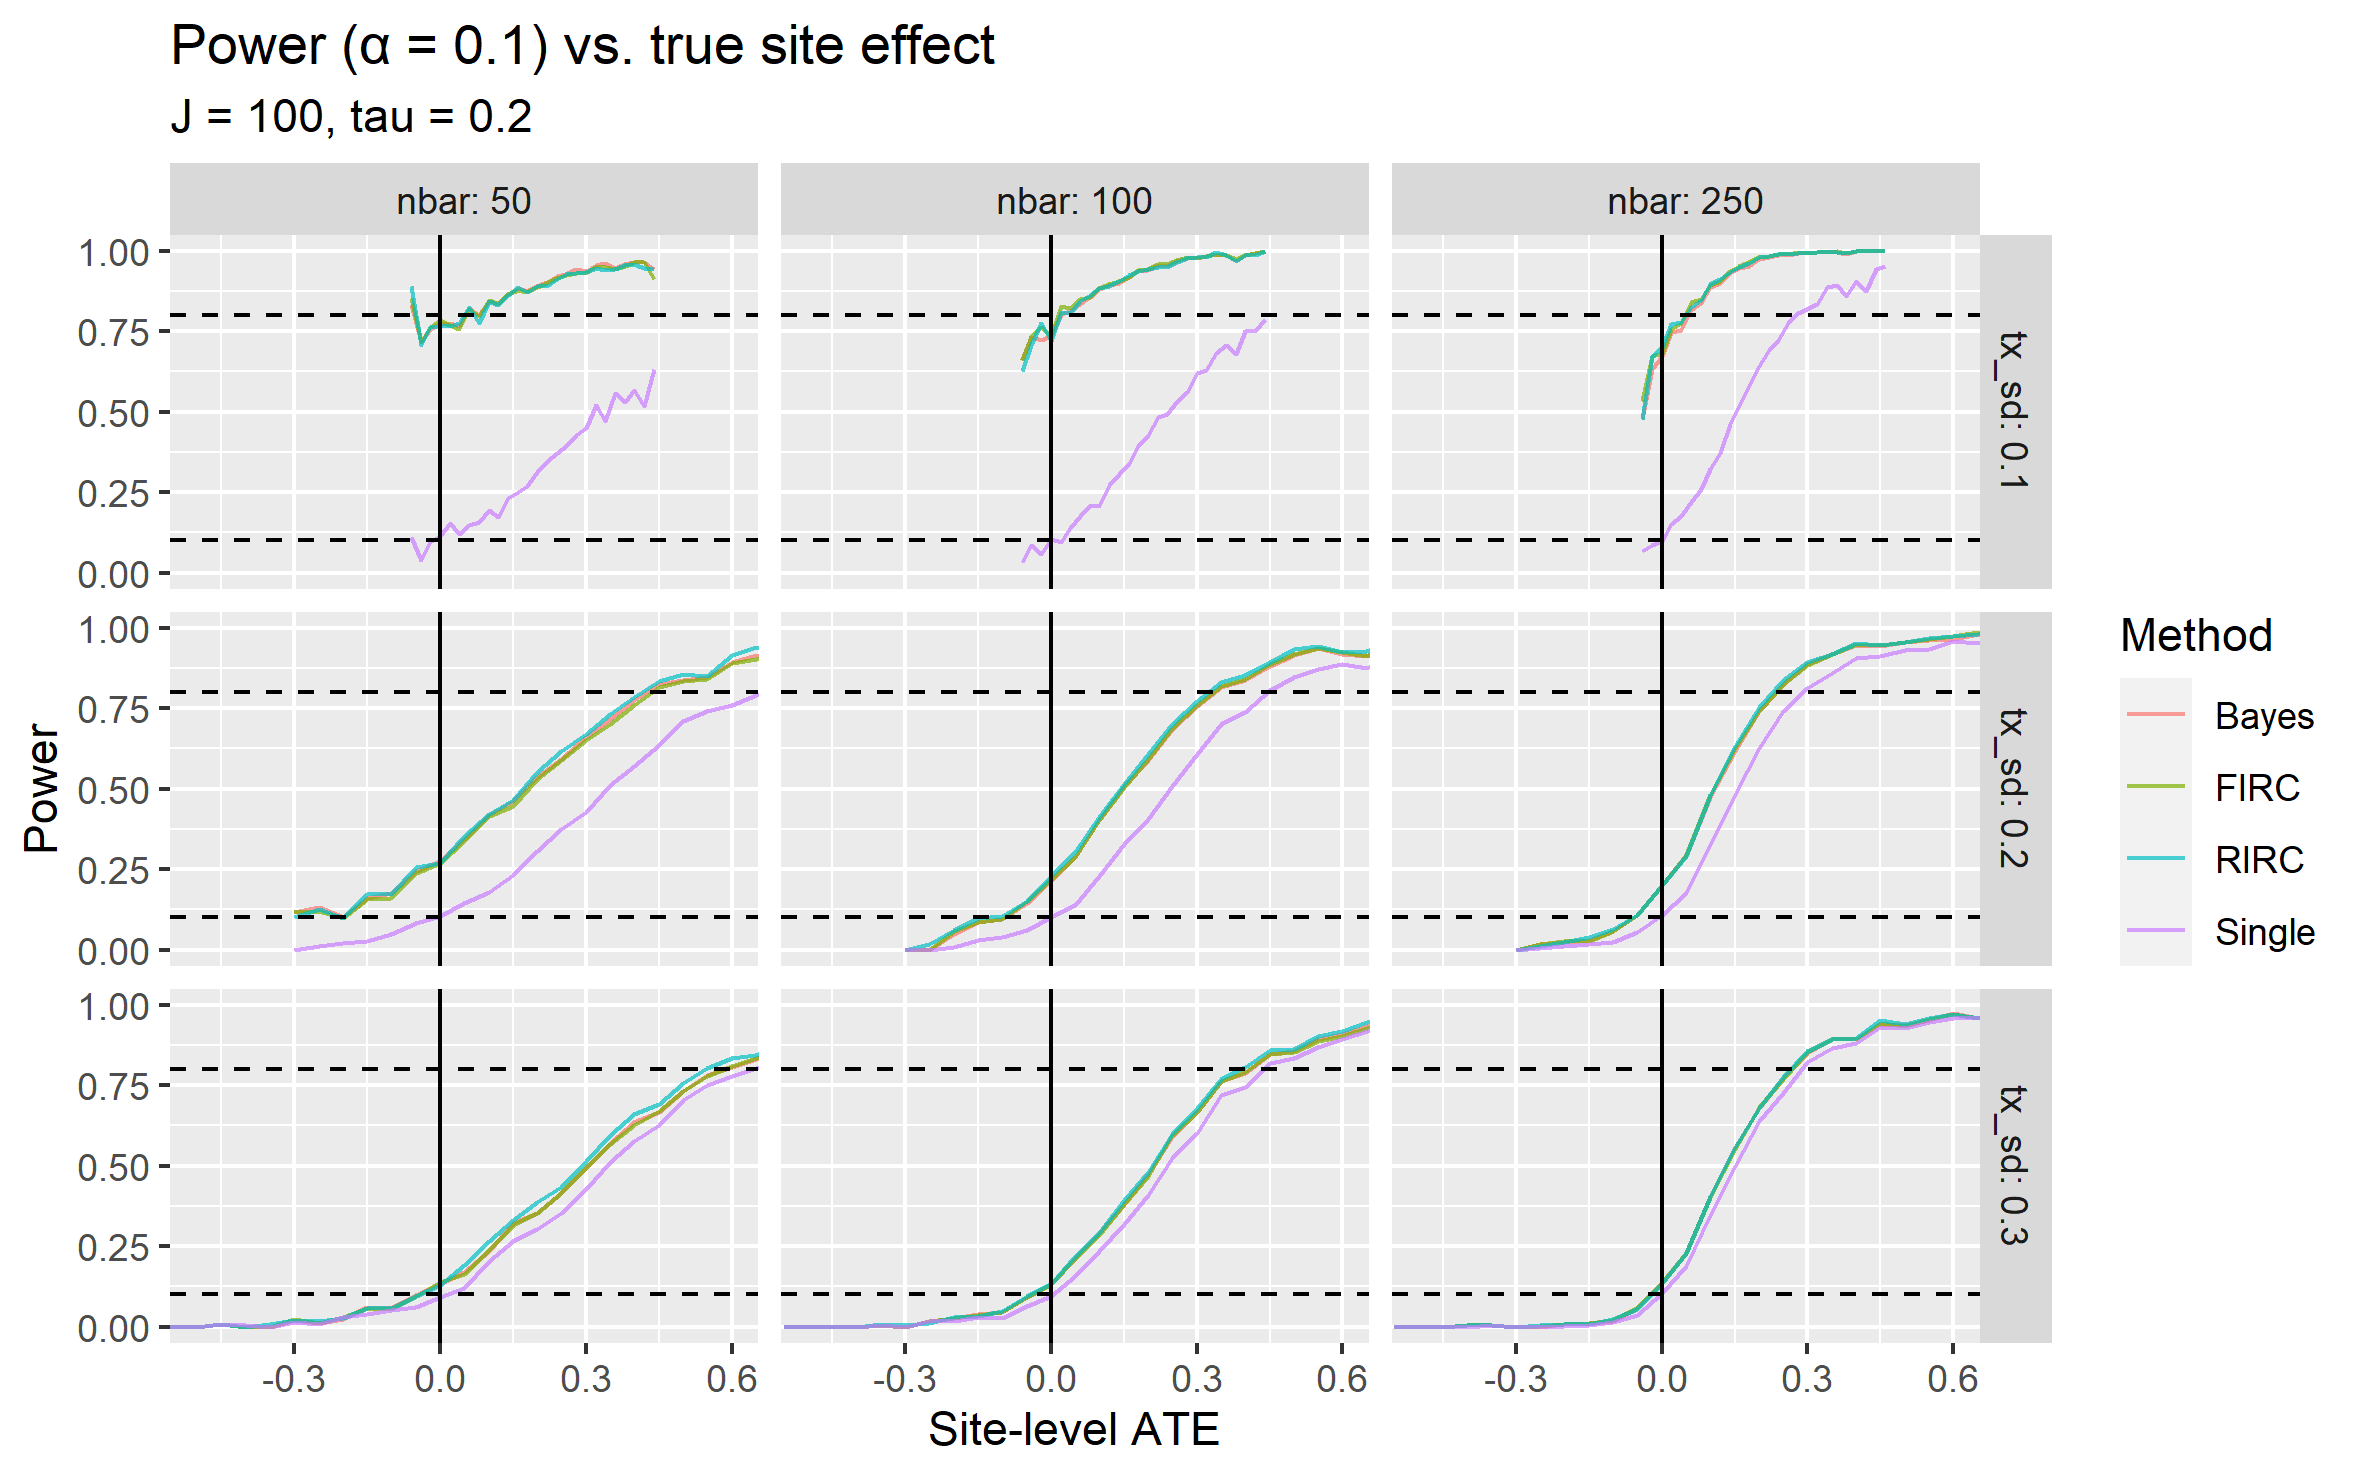
\includegraphics[width=\textwidth]{power_plot_J100}
	\caption{Power (at $\alpha = 0.1$) vs. true site ATE}
	\label{fig:power_plot}
\end{figure}

We see that while using MLMs improve power relative to estimating each site separately, these improvements often come at the cost of test validity.
This result holds for all of the MLMs in all settings, and is particularly extreme when cross-site variation is low ($\sigma_\tau = 0.1$), where the false positive rate for sites with negative $\tau_j$ values is nearly 80\%.

This behavior is expected for MLMs when power is computed at fixed values of $\tau_j$: MLMs naturally shrink estimates for sites with unusually small $\tau_j$ values toward the estimated overall mean, which is closer to $\tau = 0.2$.
The MLMs therefore estimate more positive effects for sites with negative $\tau_j$ values, resulting in many false rejections, particularly when the amount of cross-site impact variation is estimated to be small, causing shrinkage to be strong.
This naturally results in interval undercoverage (and falsely inflated power) for sites with true $\tau_j$ values far from the overall mean, as demonstrated in Figure \ref{fig:coverage_plot}.
\begin{figure}[ht]
	\centering
	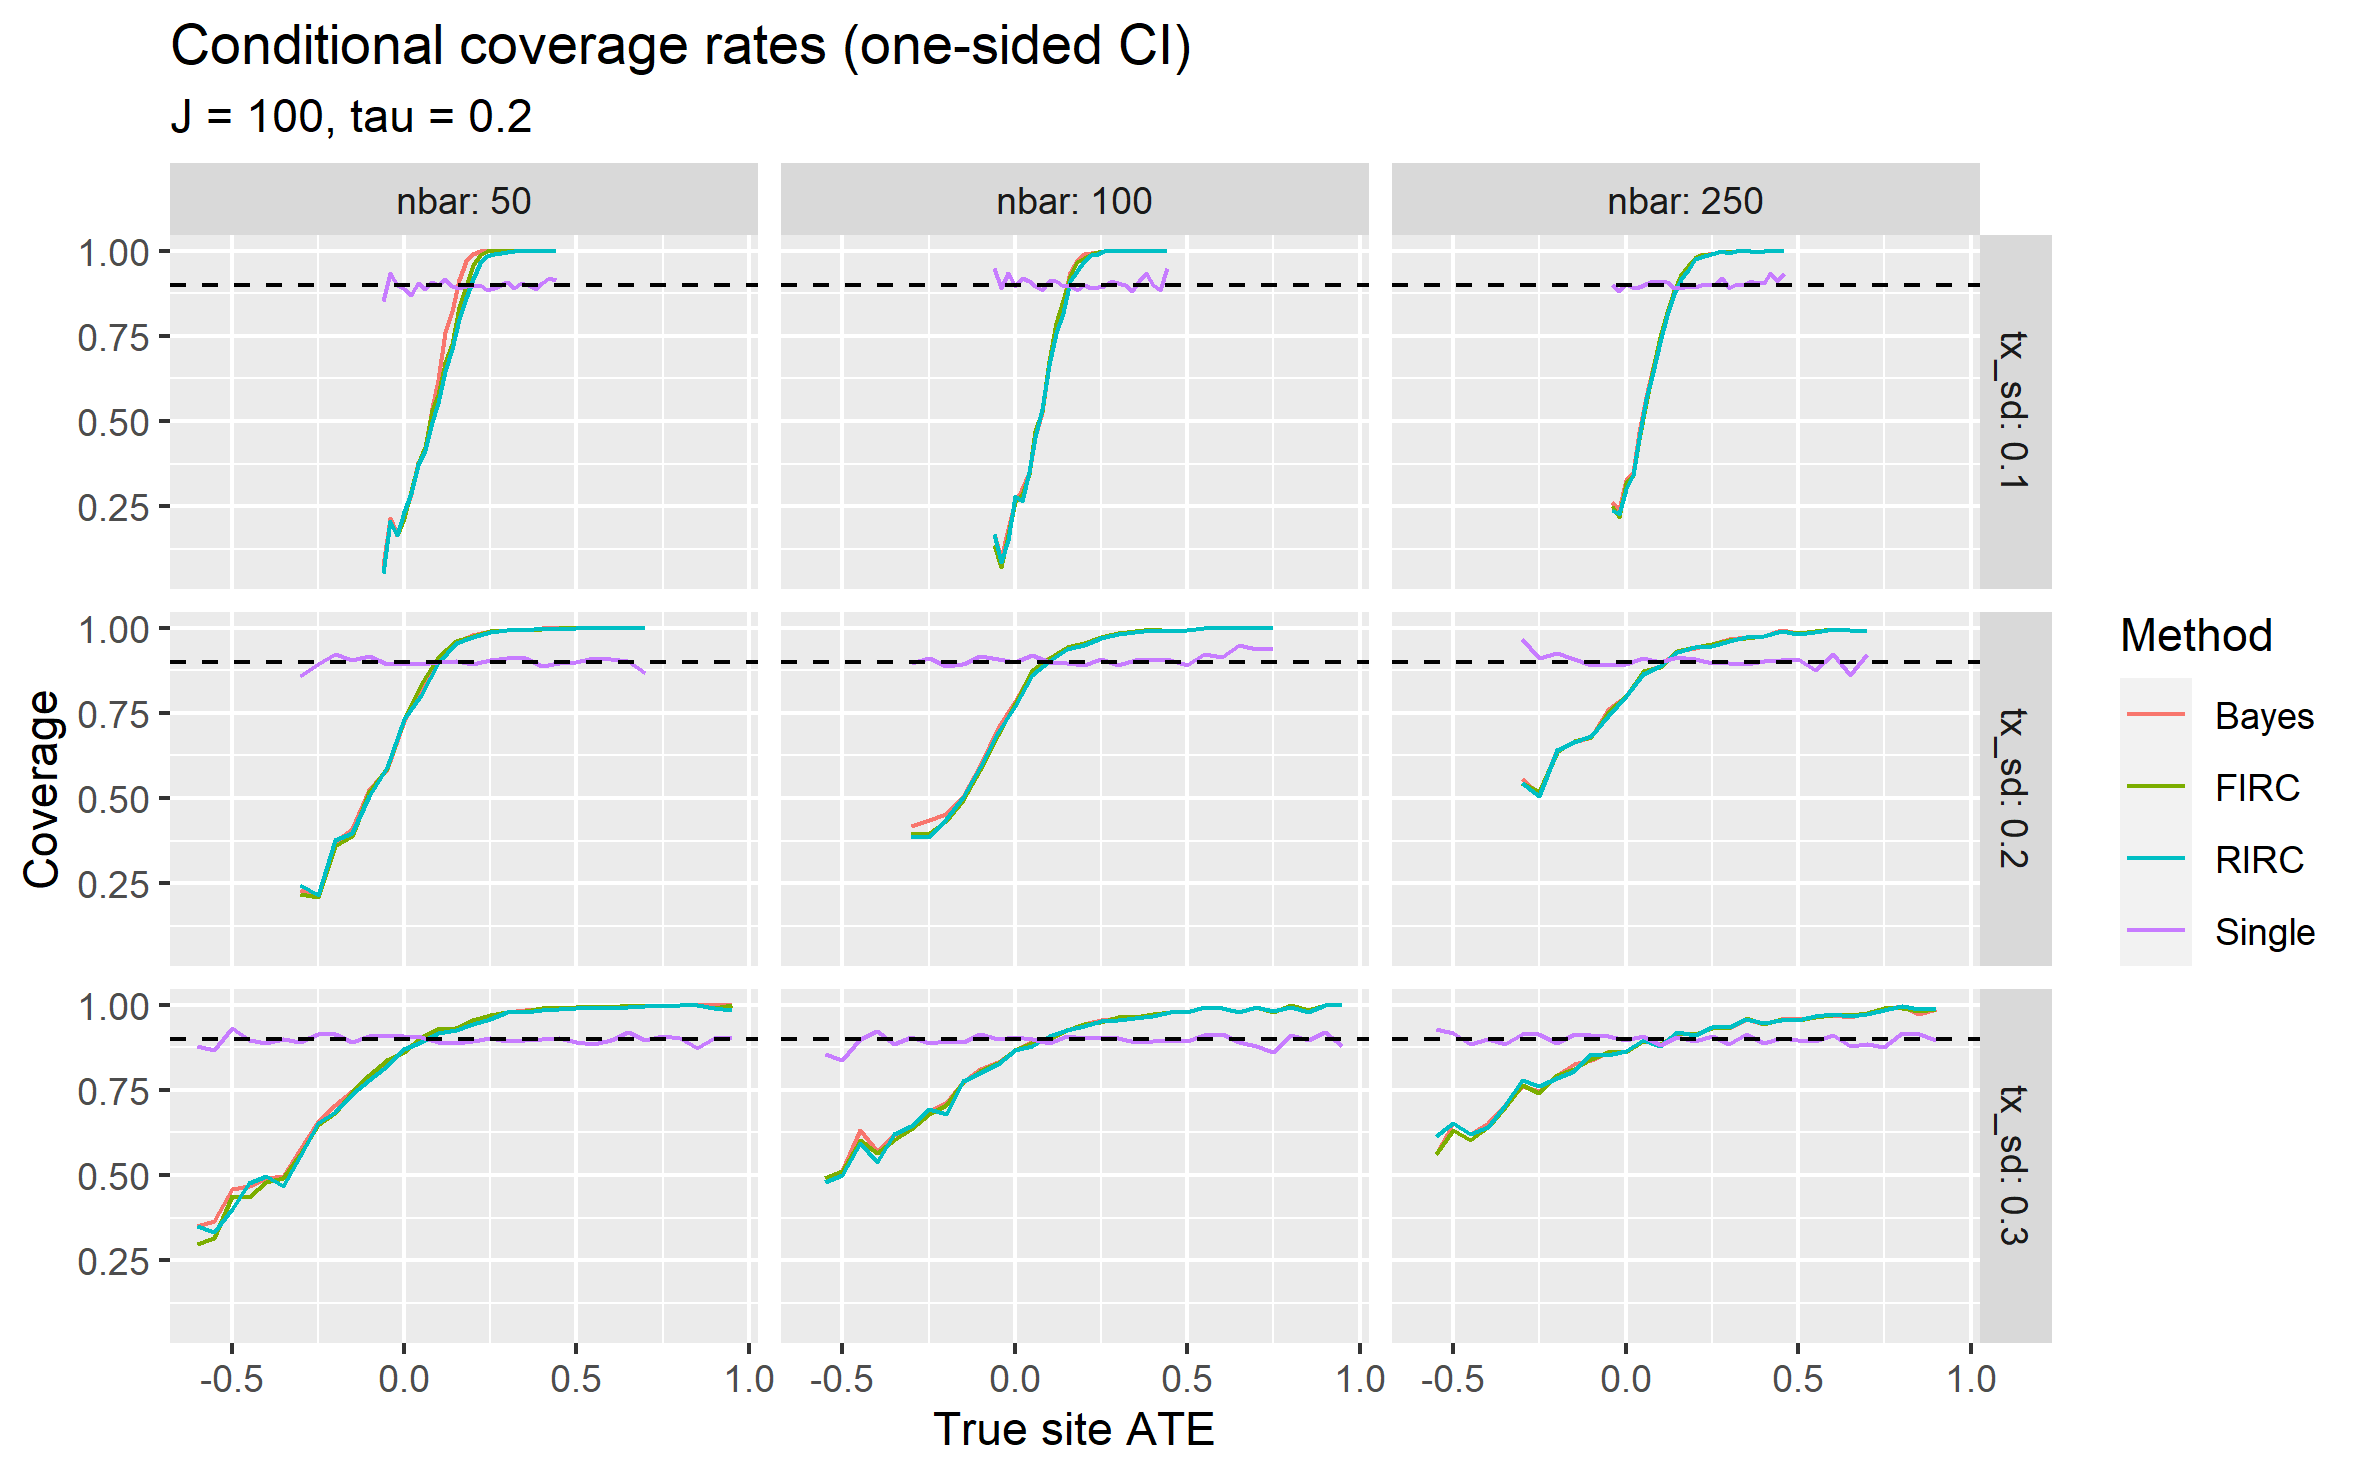
\includegraphics[width=\textwidth]{writeup/images/coverage_plot.png}
	\caption{Coverage (at $\alpha = 0.1$) vs. true site ATE}
	\label{fig:coverage_plot}
\end{figure}

In other words, MLMs have poor Frequentist coverage properties for fixed $\tau_j$ values, unlike running separate t-tests for each site.
Even when MLMs are well-specified (as they are in our simulations), their Bayesian credible intervals on $\hat{\tau}_j$ are designed to have proper Empirical Bayes coverage rates for $\tau_j$ \textit{on average}, across the prior distribution of true $\tau_j$ values, and not for any single, fixed $\tau_j$ value.
%\footnote{We note that in our simulations, Bayesian intervals indeed achieve roughly nominal Empirical Bayes coverage rates in most cases, except when shrinkage is very strong (e.g., low $\bar{n}$ and low $\sigma_\tau$).}
A naive power analysis that posits an effect size $\tau_j^*$ that the analyst would like to detect therefore leads to unsatisfactory results, since Bayesian notions of power and coverage are not defined conditional on fixed values of $\tau_j$.

Instead of naive Frequentist power analyses, we propose that analysts may conduct prospective interval-length analyses.
Using the simulation framework in this paper, an analyst can size a study to achieve a particular average interval width, across sites.
Figure \ref{fig:length_plot} demonstrates an example of this analysis.
\begin{figure}[ht]
	\centering
	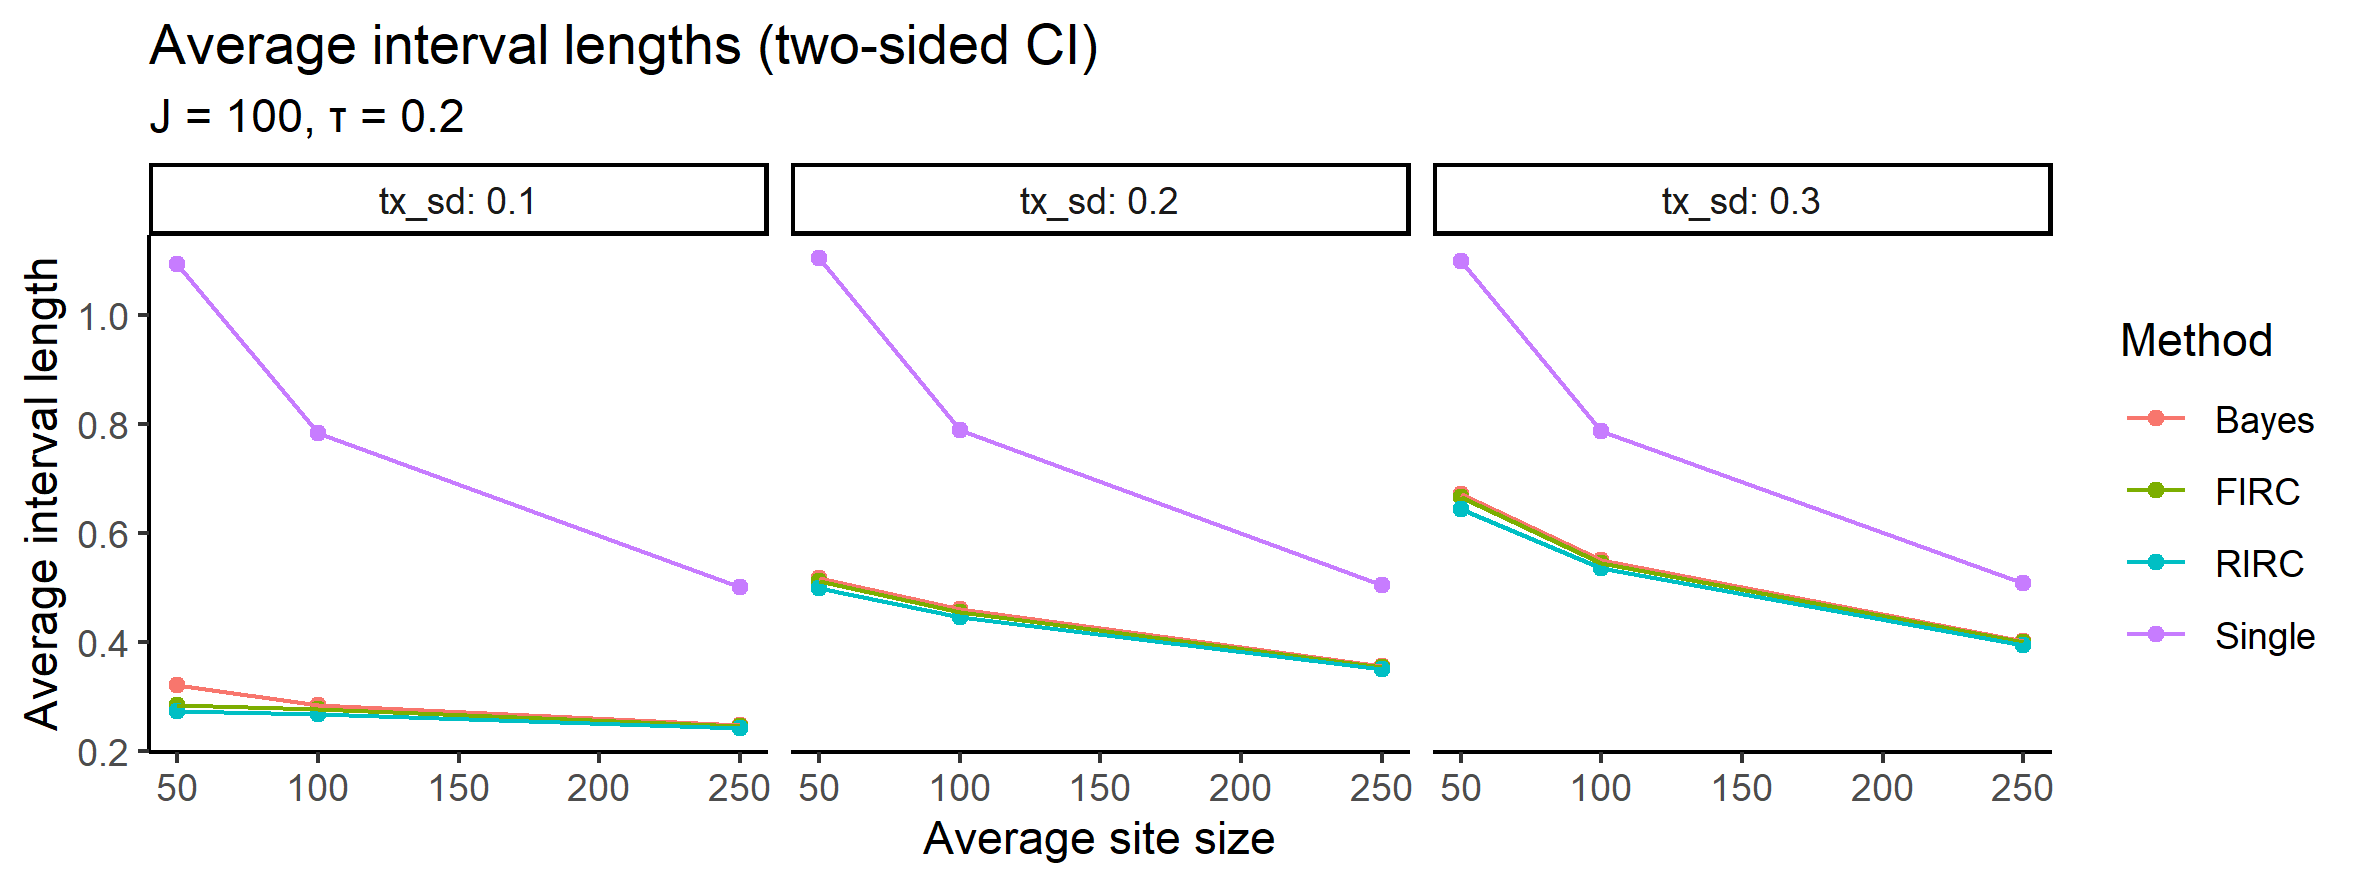
\includegraphics[width=\textwidth]{writeup/images/length_plot.png}
	\caption{Average two-sided credible interval length (at $\alpha = 0.1$)}
	\label{fig:length_plot}
\end{figure}
We see that using MLMs significantly decreases average interval length, particularly when $\sigma_\tau$ is small (i.e., shrinkage is high).
If, for example, an interval length of 0.4 is desirable for site stakeholders and treatment-effect variation is expected to be moderate ($\sigma_\tau$ = 0.2), an analyst may note that the 100 sites would have to reasonably large ($\bar{n} \approx 250$) in order to achieve the desired interval length on average.

% MLMs, however, have excellent coverage properties and power \textit{for fixed $\hat{\tau}_j$ values} when they are well-specified.
% Figure \ref{fig:power_plot_cond} replicates Figure \ref{fig:power_plot}, except now test powers (i.e., rejection rates) are computed for fixed $\hat{\tau}_j$ values rather than for fixed $\tau_j$ values.
% \begin{figure}[ht]
% 	\centering
% 	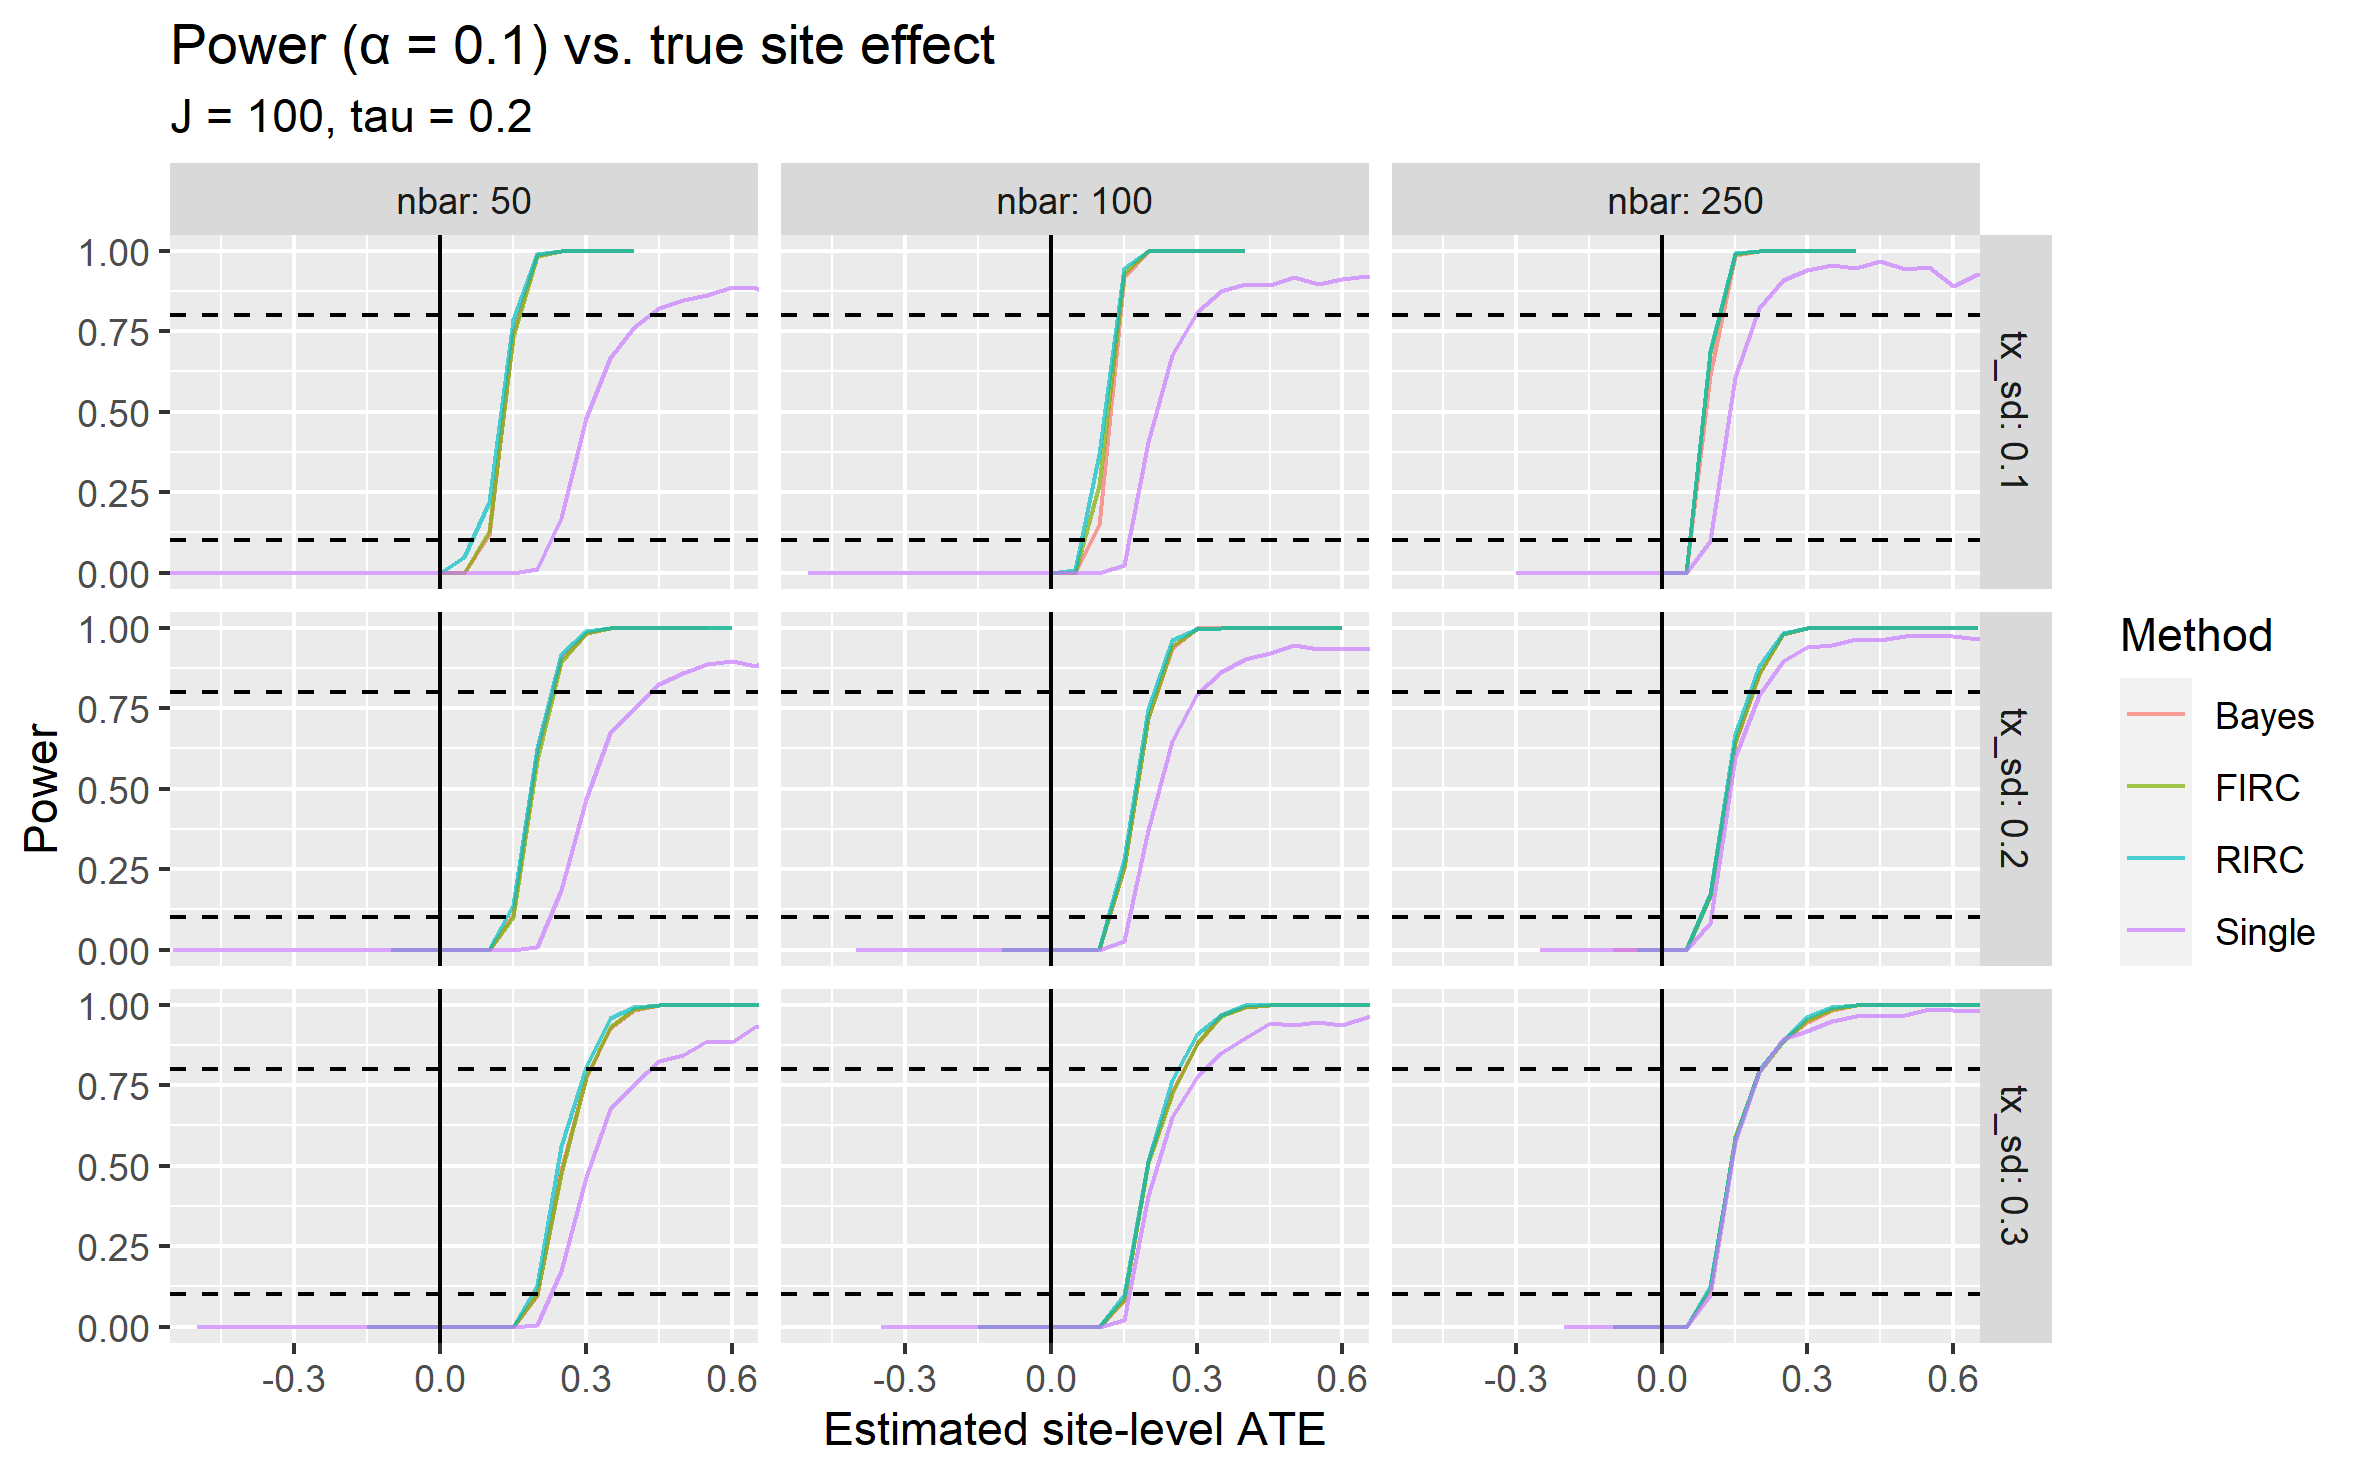
\includegraphics[width=\textwidth]{cond_power_1sided}
% 	\caption{Power (at $\alpha = 0.1$) vs. estimated site ATE}
% 	\label{fig:power_plot_cond}
% \end{figure}
% Under this setup, we see that the MLMs have significantly greater power than the individual t-tests.
% Figure \ref{fig:coverage_plot_cond} also shows that the coverage rates for the MLMs are generally correct.
% \begin{figure}[ht]
% 	\centering
% 	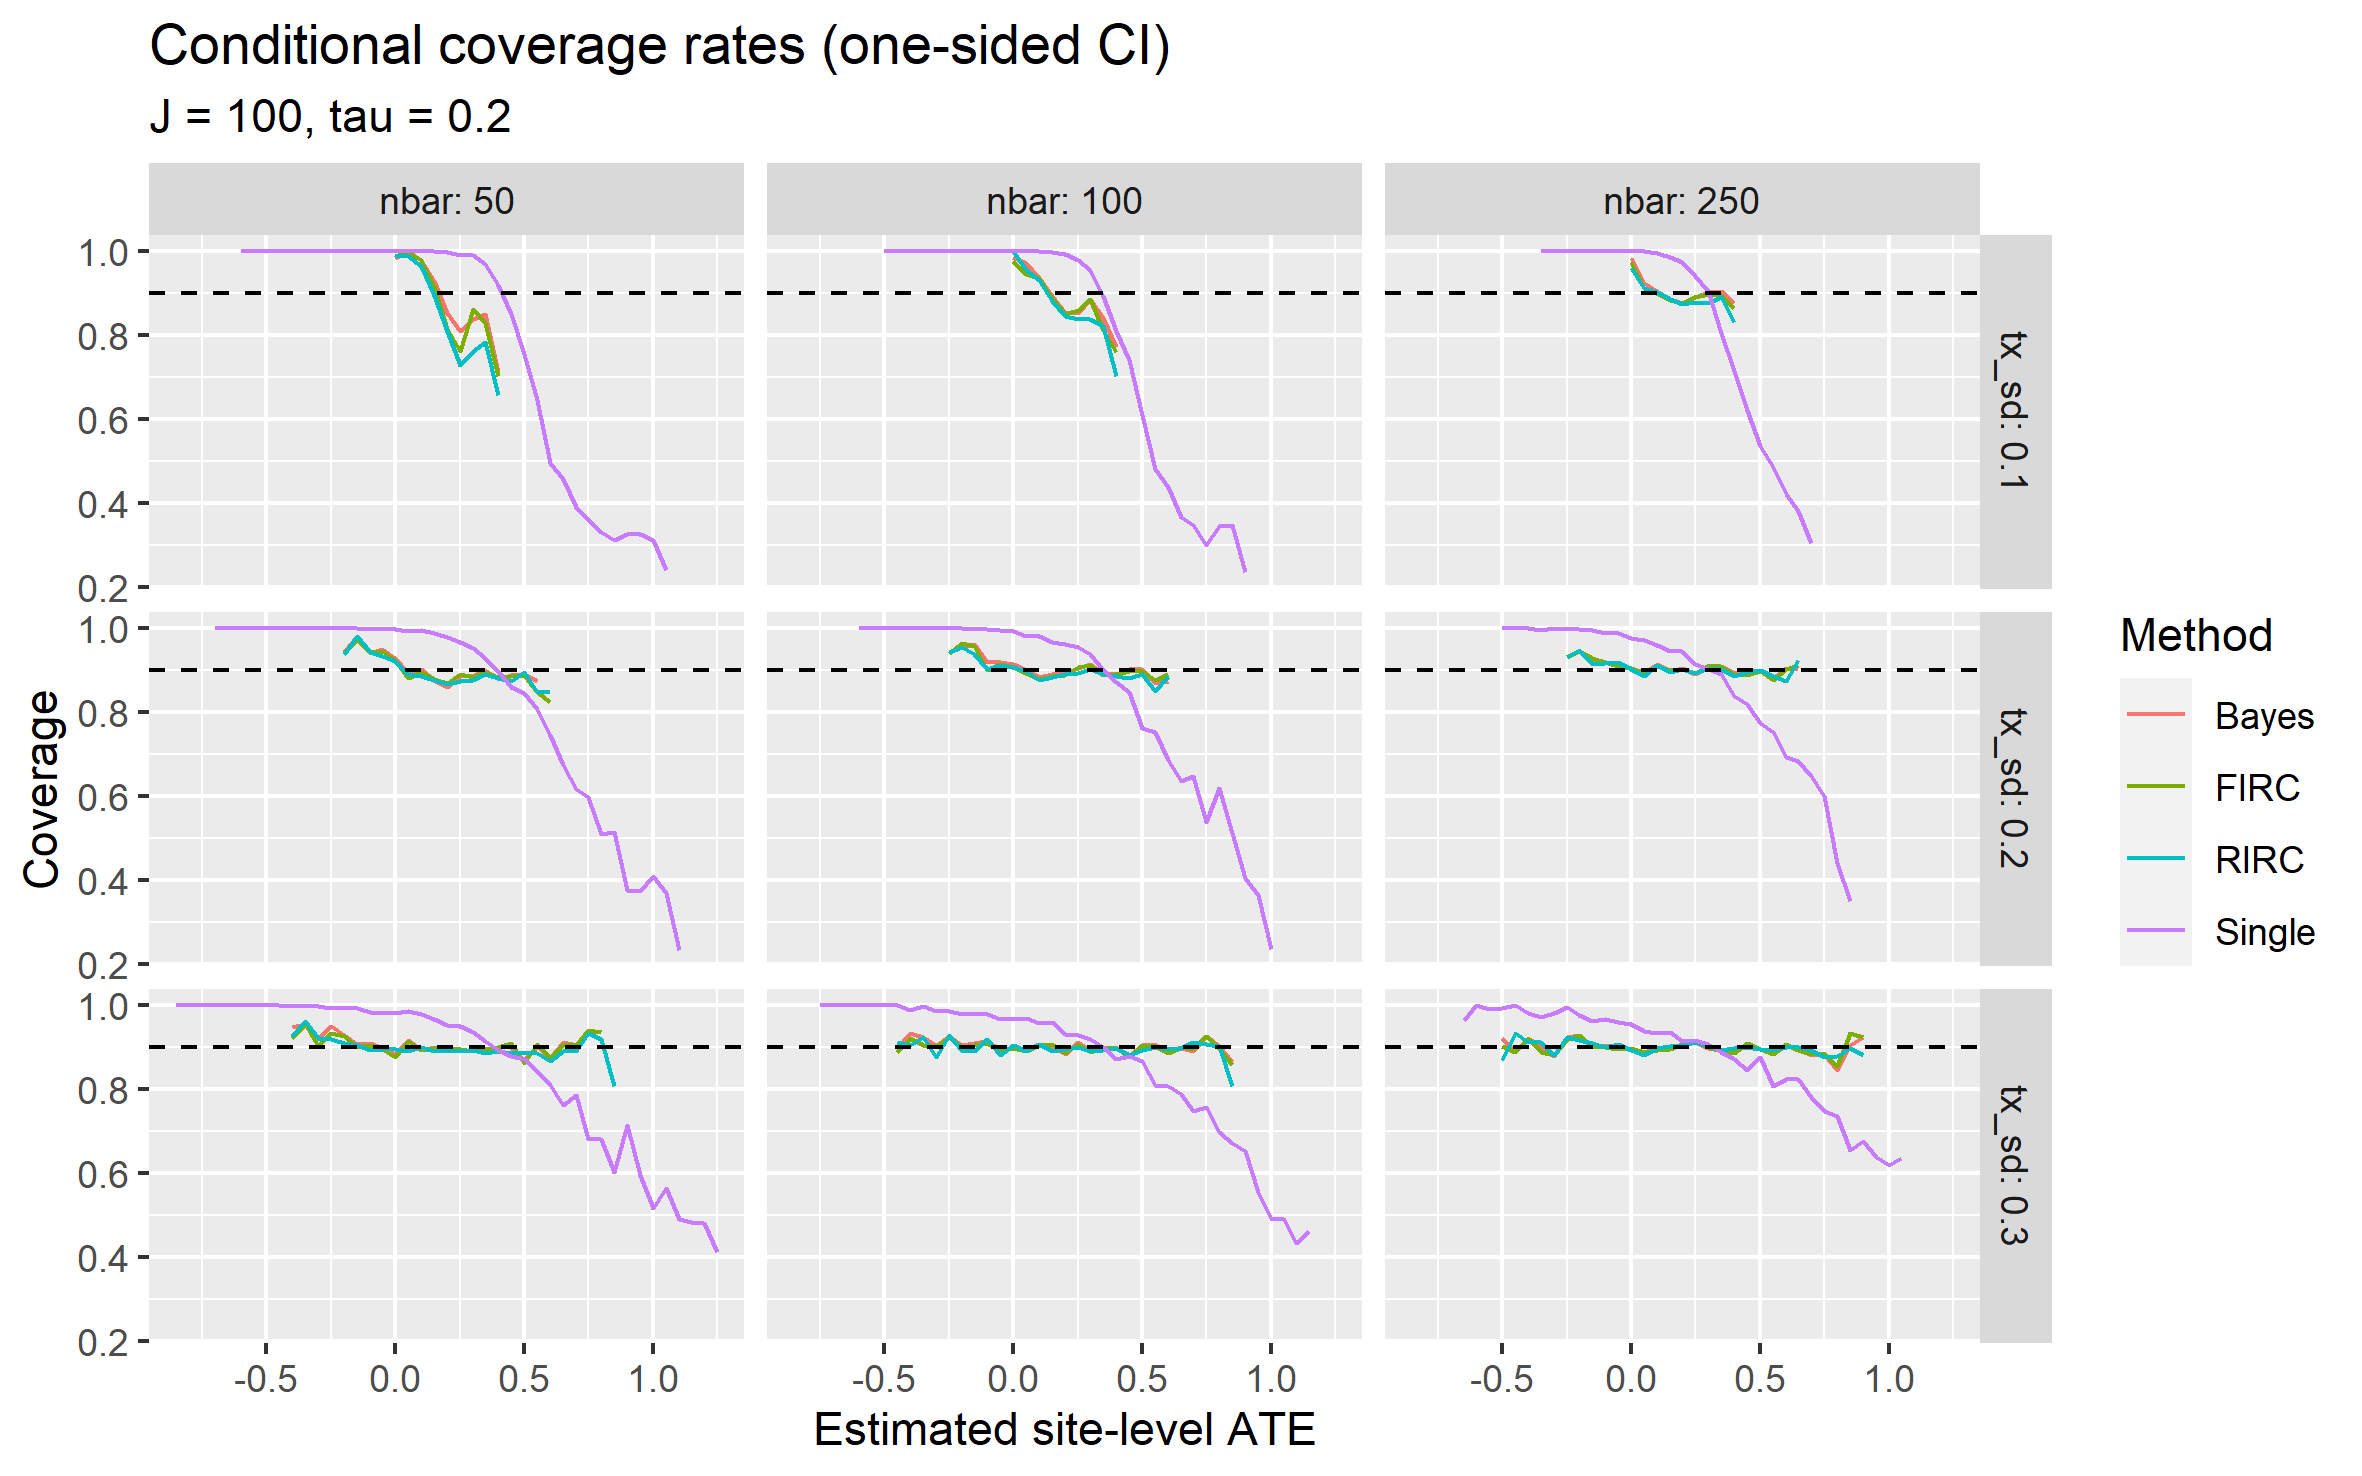
\includegraphics[width=\textwidth]{writeup/images/cond_coverage_1sided.png}
% 	\caption{Coverage (at $\alpha = 0.1$) vs. estimated site ATE}
% 	\label{fig:coverage_plot_cond}
% \end{figure}

% The results in Figures \ref{fig:power_plot_cond} and \ref{fig:coverage_plot_cond} are due to the MLMs appropriately shrinking extreme site-level effect estimates.
% Estimated site-level effects $\hat{\tau}_j$ may be extreme either because $\tau_j$ is extreme or because of random noise.
% MLMs use shrinkage to account for the fact that the majority of extreme $\hat{\tau}_j$ estimates are due to random noise rather than actual extreme signals; as a result, we see in our simulations that they produce intervals with better coverage rates than do individual site t-tests, particularly for large $\hat{\tau}_j$ values.
% Shrinkage also results in narrower intervals for sites with $\hat{\tau}_j$ close to the estimated overall average treatment effect, which improves power for those sites.


\section{Conclusions}

In many multisite trials, analysts may wish to power the trial to allow consistent detection of particular effect sizes at individual sites.
The credible intervals generated by MLMs, however, only guarantee average coverage rates across all sites, and not for sites with a fixed effect size $\tau_j$.
As a result, naive Frequentist power analyses for fixed $\tau_j$ values indicate that while MLMs have more power for detecting effects at individual sites than does separately testing each site, they are generally invalid.
Rather than performing naive Frequentist power analyses, analysts may consider running average-interval-length analyses.
Using the simulation framework in this paper, analysts may size a prospective study to achieve an average interval-length that stakeholders would be satisfied with for their individual site-level inferences.


\bibliography{refs.bib}
	
\end{document}